%----------------------------------------------------------------------------------------
%	PACKAGES AND OTHER DOCUMENT CONFIGURATIONS
%----------------------------------------------------------------------------------------

\documentclass[paper=a4, fontsize=11pt]{scrartcl} % A4 paper and 11pt font size

\usepackage[margin=1.0in]{geometry}	%for some reason, looks beter. 

\usepackage[T1]{fontenc} % Use 8-bit encoding that has 256 glyphs
\usepackage{fourier} % Use the Adobe Utopia font for the document - comment this line to return to the LaTeX default
\usepackage[english]{babel} % English language/hyphenation
\usepackage{amsmath,amsfonts,amsthm} % Math packages

\usepackage{lipsum} % Used for inserting dummy 'Lorem ipsum' text into the template

\usepackage{sectsty} % Allows customizing section commands
\allsectionsfont{\centering \normalfont\scshape} % Make all sections centered, the default font and small caps

\usepackage{fancyhdr} % Custom headers and footers
\pagestyle{fancyplain} % Makes all pages in the document conform to the custom headers and footers
\fancyhead{} % No page header - if you want one, create it in the same way as the footers below
\fancyfoot[L]{} % Empty left footer
\fancyfoot[C]{} % Empty center footer
\fancyfoot[R]{\thepage} % Page numbering for right footer
\renewcommand{\headrulewidth}{0pt} % Remove header underlines
\renewcommand{\footrulewidth}{0pt} % Remove footer underlines
\setlength{\headheight}{13.6pt} % Customize the height of the header

\numberwithin{equation}{section} % Number equations within sections (i.e. 1.1, 1.2, 2.1, 2.2 instead of 1, 2, 3, 4)
\numberwithin{figure}{section} % Number figures within sections (i.e. 1.1, 1.2, 2.1, 2.2 instead of 1, 2, 3, 4)
\numberwithin{table}{section} % Number tables within sections (i.e. 1.1, 1.2, 2.1, 2.2 instead of 1, 2, 3, 4)

\setlength\parindent{0pt} % Removes all indentation from paragraphs - comment this line for an assignment with lots of text

%----------------------------------------------------------------------------------------
%Personal Packages and File Dependencies 
%----------------------------------------------------------------------------------------	

\usepackage{graphicx}	%insert graphics
\usepackage{microtype}	%improves spacing
\usepackage{float}		%H postion	
\usepackage{caption}	%caption w/o : 	
\usepackage{framed}		%creates frames
\usepackage{enumitem}
\usepackage{nag}

\usepackage{listings}	%insert sourcecode
\usepackage{color}
\usepackage{pdfpages}	%include PDF pages

\usepackage{bigstrut}	%exce2latex table packages
\usepackage{rotating}
\usepackage{multirow}
\usepackage{booktabs}
%\usepackage[framed]{mcode}

\usepackage{cleveref}	%cooler references, needs to be last
\usepackage[bookmarks]{hyperref}
\graphicspath{{../Figures/}{../figures/}} % This automatically connects to the figure folder

%----------------------------------------------------------------------------------------
%	TITLE SECTION
%----------------------------------------------------------------------------------------

\newcommand{\horrule}[1]{\rule{\linewidth}{#1}} % Create horizontal rule command with 1 argument of height

\title{	
\normalfont \normalsize 
\textsc{TEMPLE UNIVERSITY COLLEGE OF ENGINEERING | ECE 3623 | SPRING 2015} \\ [25pt] % Your university, school and/or department name(s)
\horrule{0.5pt} \\[0.4cm] % Thin top horizontal rule
\huge Embedded Systems Lab 1: Regression and Histograms \\ % The assignment title
\horrule{2pt} \\[0.5cm] % Thick bottom horizontal rule
}

\author{Tyler Berezowsky} % Your name

\date{\normalsize\today} % Today's date or a custom date 
\usepackage{mcode}

\begin{document}
\maketitle % Print the title

\section{Problem Statement} 
%Summarize the problem statement in one paragraph. Clearly state what the knowns are and what unknowns you must find.
The goal of this assignment is to introduce covariance and correlation calculations. For this task, only the audio signal was used. The tasks to be accomplished are:
\begin{enumerate}
\item Define a vector, x, of length 240 (30 msec) that contains the 240 samples of the signal starting at $t=0.9$ secs. Define a second vector, y, which also represents 240 samples, but consists of samples shifted by k samples (e.g., k = 1 implies y starts one sample later than x). Plot the statistical correlation between x and y for k = 0, 1, ..., 512. Can you explain what you observe? (Hint: think about what would happen if the signal were a sinewave.)\\

Repeat this for t = 3.0 secs. Compare the two functions and relate them to properties of the audio signal.\\

The function you are plotting is known as the autocorrelation function. It is a minimum phase version of the actual signal. You can learn more about that in a course on digital signal processing.

\item Again, start at $t=0.9$ secs. Take the first 16 samples as a vector: $x = [x_1, x_2, x_3, ..., x_{16}]$. Compute the covariance matrix using 240 samples. Each element in the matrix is governed by the equation:
\begin{equation}
x[i,j] = \frac{1}{N}\sum_{n=0}^{N-1} x[n-i]x[n-j]
\end{equation}

where i is defined over the range [0, 15] and j is defined over the range [0, 15]. Do this for t = 1.1 secs and t = 3.0 secs. Compare the two matrices and explain why they are different.
\end{enumerate}
\section{Approach and Results} 
%Describe your approach to finding the unknowns. Use numbered figures, tables and equations where necessary.

\subsection{Correlation}  
The correlation coefficient is defined by equation~\ref{eq: coeff}. It consists the covariance of two random variables divided by the standard deviation of each variable multiplied. This reduces the range of covariance to -1 and 1. 
\begin{equation}
\rho_{XY} = \frac{E[(X-\mu_X)(Y-\mu_Y)]}{\sqrt{Var(X)Var(Y)}}
\label{eq: coeff}
\end{equation}
The correlation coefficient provides a metric to determine how linearly related two random variables are. If the coefficient is negative 1, they are inversely related. If the coefficient is a positive one, they are directly related. A coefficient of  zero states that the variables are not linearly correlated. Note that this does not mean they are not correlated at a higher power.  \\ 

For task 1, the correlation of a vector, $x$ ,from the provided audio signal was taken against itself,  $y$, but shifted by $k$ bits. ($k$ = 512) The starting time of x was equal to $x_1 = 0.9$, $x_2 = 1.1$, and $x_3 = 3.0$ seconds. The resulting correlation coefficients were plotted against their respective $k$ value. The plots for offsets $x_1$, $x_2 $, and $x_3$ can be seen in figure~\ref{fig: correlation}.


\begin{figure}[H] 
	\centering 
	\includegraphics[width=\linewidth]{plot_1.eps}
	\caption{Correlation of audio signal vector $x$ starting at offset $x_i$ with itself shifted by $k$ bits. Offset $x_1 = 0.9s$, $x_2 = 1.1s$, and $x_3 = 3.0s$}
	\label{fig: correlation} 
\end{figure}

For every offset value, the correlation coefficient begins with 1 as $k$ starts at 0. This compares the $x$ vector with the un-shifted version of itself, therefore the correlation is 1. Offset $x_1$ decays after $k=0$ with periodic pulses. Offset $x_2$ also decays after $k=0$ with random peaks. Offset $x_3$ decays after $k=0$ substantially faster than $x_1$ and $x_2$ and remains under 0.5 to -0.5 for the duration of the rest of the signal. 

\subsection{Covariance Matrix} 
The covariance matrices for offsets $x_0 = 0.9$, $x_1 = 1.1$, and $x_2 = 3.0$ seconds are respectively displayed below. The covariance matrix computes the covariance between the $i$th and $j$th elements of the applied vector. Therefore, when $i = j$ the same elements in the vector are being compared and should represent the maximum value of covariance between elements in the matrix. Due to distribution of the elements, all covariance matrices are also symmetrical along the diagonal. This is represented in the matrices generated. 

\begin{figure}[H] 
	\centering 
	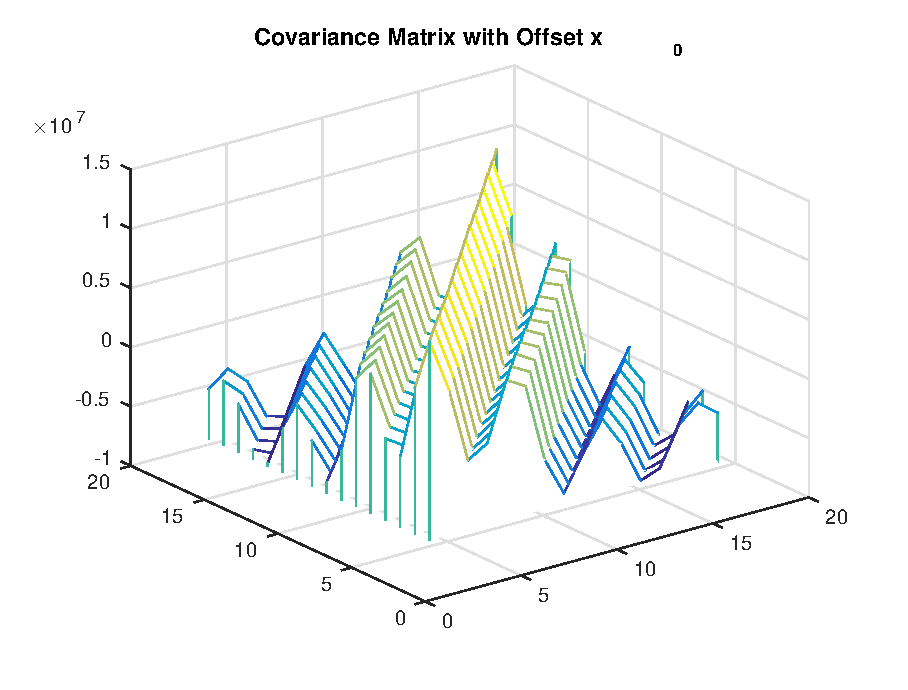
\includegraphics[width=\linewidth]{plot_2.eps}
	\caption{Covariance matrix with offset $x_0 = 0.9$ seconds.}
	\label{fig: c1} 
\end{figure}

\begin{figure}[H] 
	\centering 
	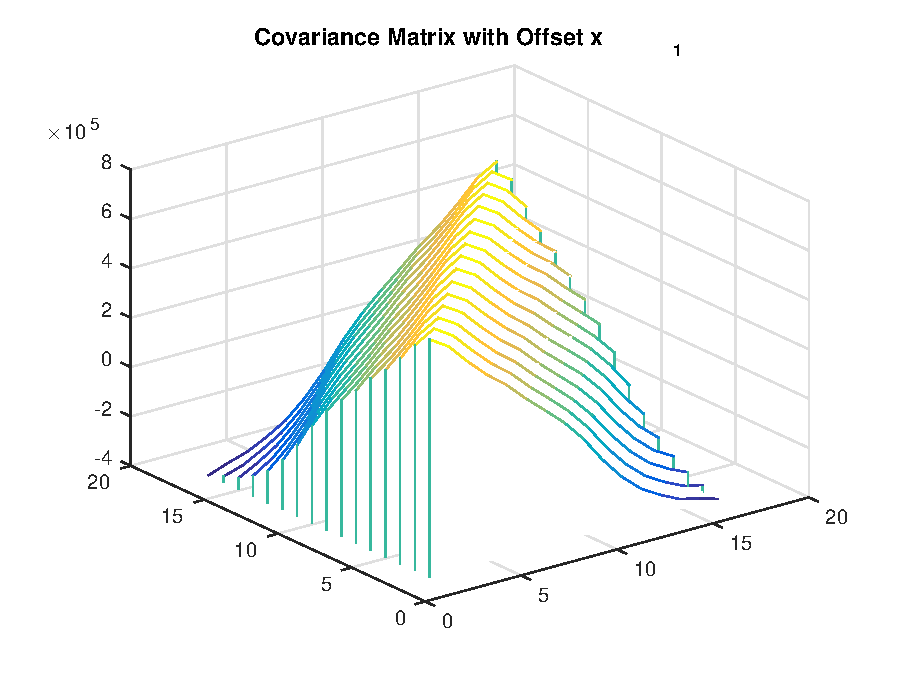
\includegraphics[width=\linewidth]{plot_3.eps}
	\caption{Covariance matrix with offset $x_1 = 1.1$ seconds.}
	\label{fig: c2} 
\end{figure}
9.
\begin{figure}[H] 
	\centering 
	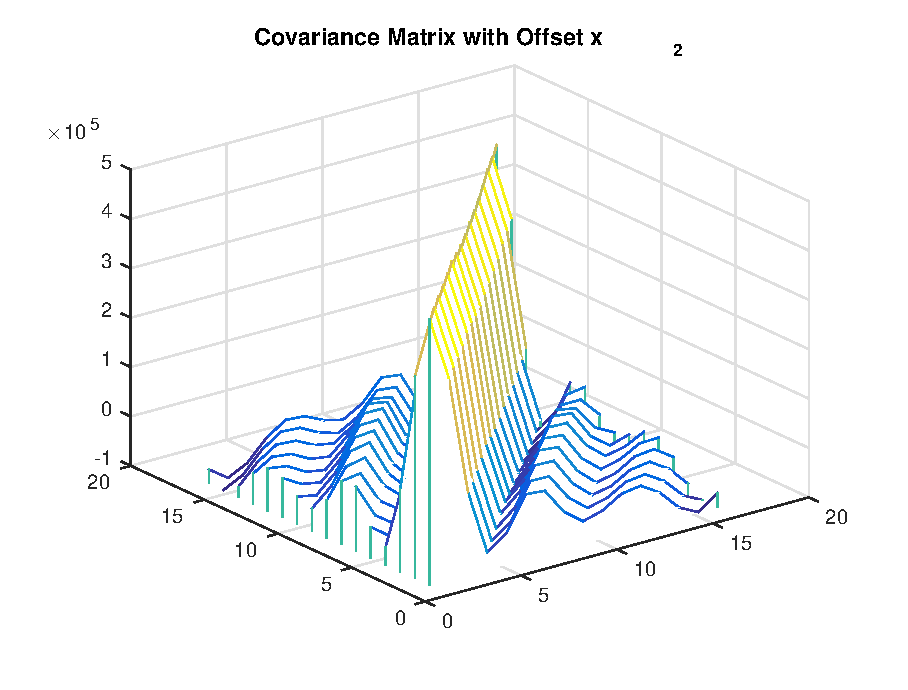
\includegraphics[width=\linewidth]{plot_4.eps}
	\caption{Covariance matrix with offset $x_2 = 3.0$ seconds.}
	\label{fig: c3} 
\end{figure}

\subsection{Spectrum Analysis} 
To further understand the distribution of covariance in the matrices, the Fourier transform of the audio vectors was taken. This provided a glimpse into the audio spectrum of each vector. The transforms are displayed in figure~\ref{fig: transform} below. \\

The frequency spectrum for $x$ with offset $x_0$ contains large peaks between 0 to 500 Hz and 1200 to 2000 Hz. The frequency spectrum for $x$ with offset $x_1$ contains most of its power under 500 Hz. The frequency spectrum for $x$ with offset $x_2$ contains peaks from 0 to 2000 Hz. \\

Attempting to bridge the gap between the audio spectrum and the covariance matrices, I'll start with the data generated by the 3.0 second offset. The audio spectrum contains various peaks from 0 to 2000Hz. The correlation matrix displays a peak along the diagonal, as to be expected, but then drops within 5 samples to near zero.  This behavior is different than the other two offsets which contain much slower decaying or oscillating decay. This suggests the signal is highly uncorrelated which is also possibly represented by the amount of energy spread across the spectrum seen in the FFT. The covariance of the other two offsets, $x_0$ and $x_1$, both drop gradually to zero. $x_0$ simply appears to do it in an oscillatory manner. The covariance should drop over time with any random audio signal, but it does not explain the oscillatory behavior for offset $x_0$ and why $x_1$ lacks it. 

\begin{figure}[H] 
	\centering 
	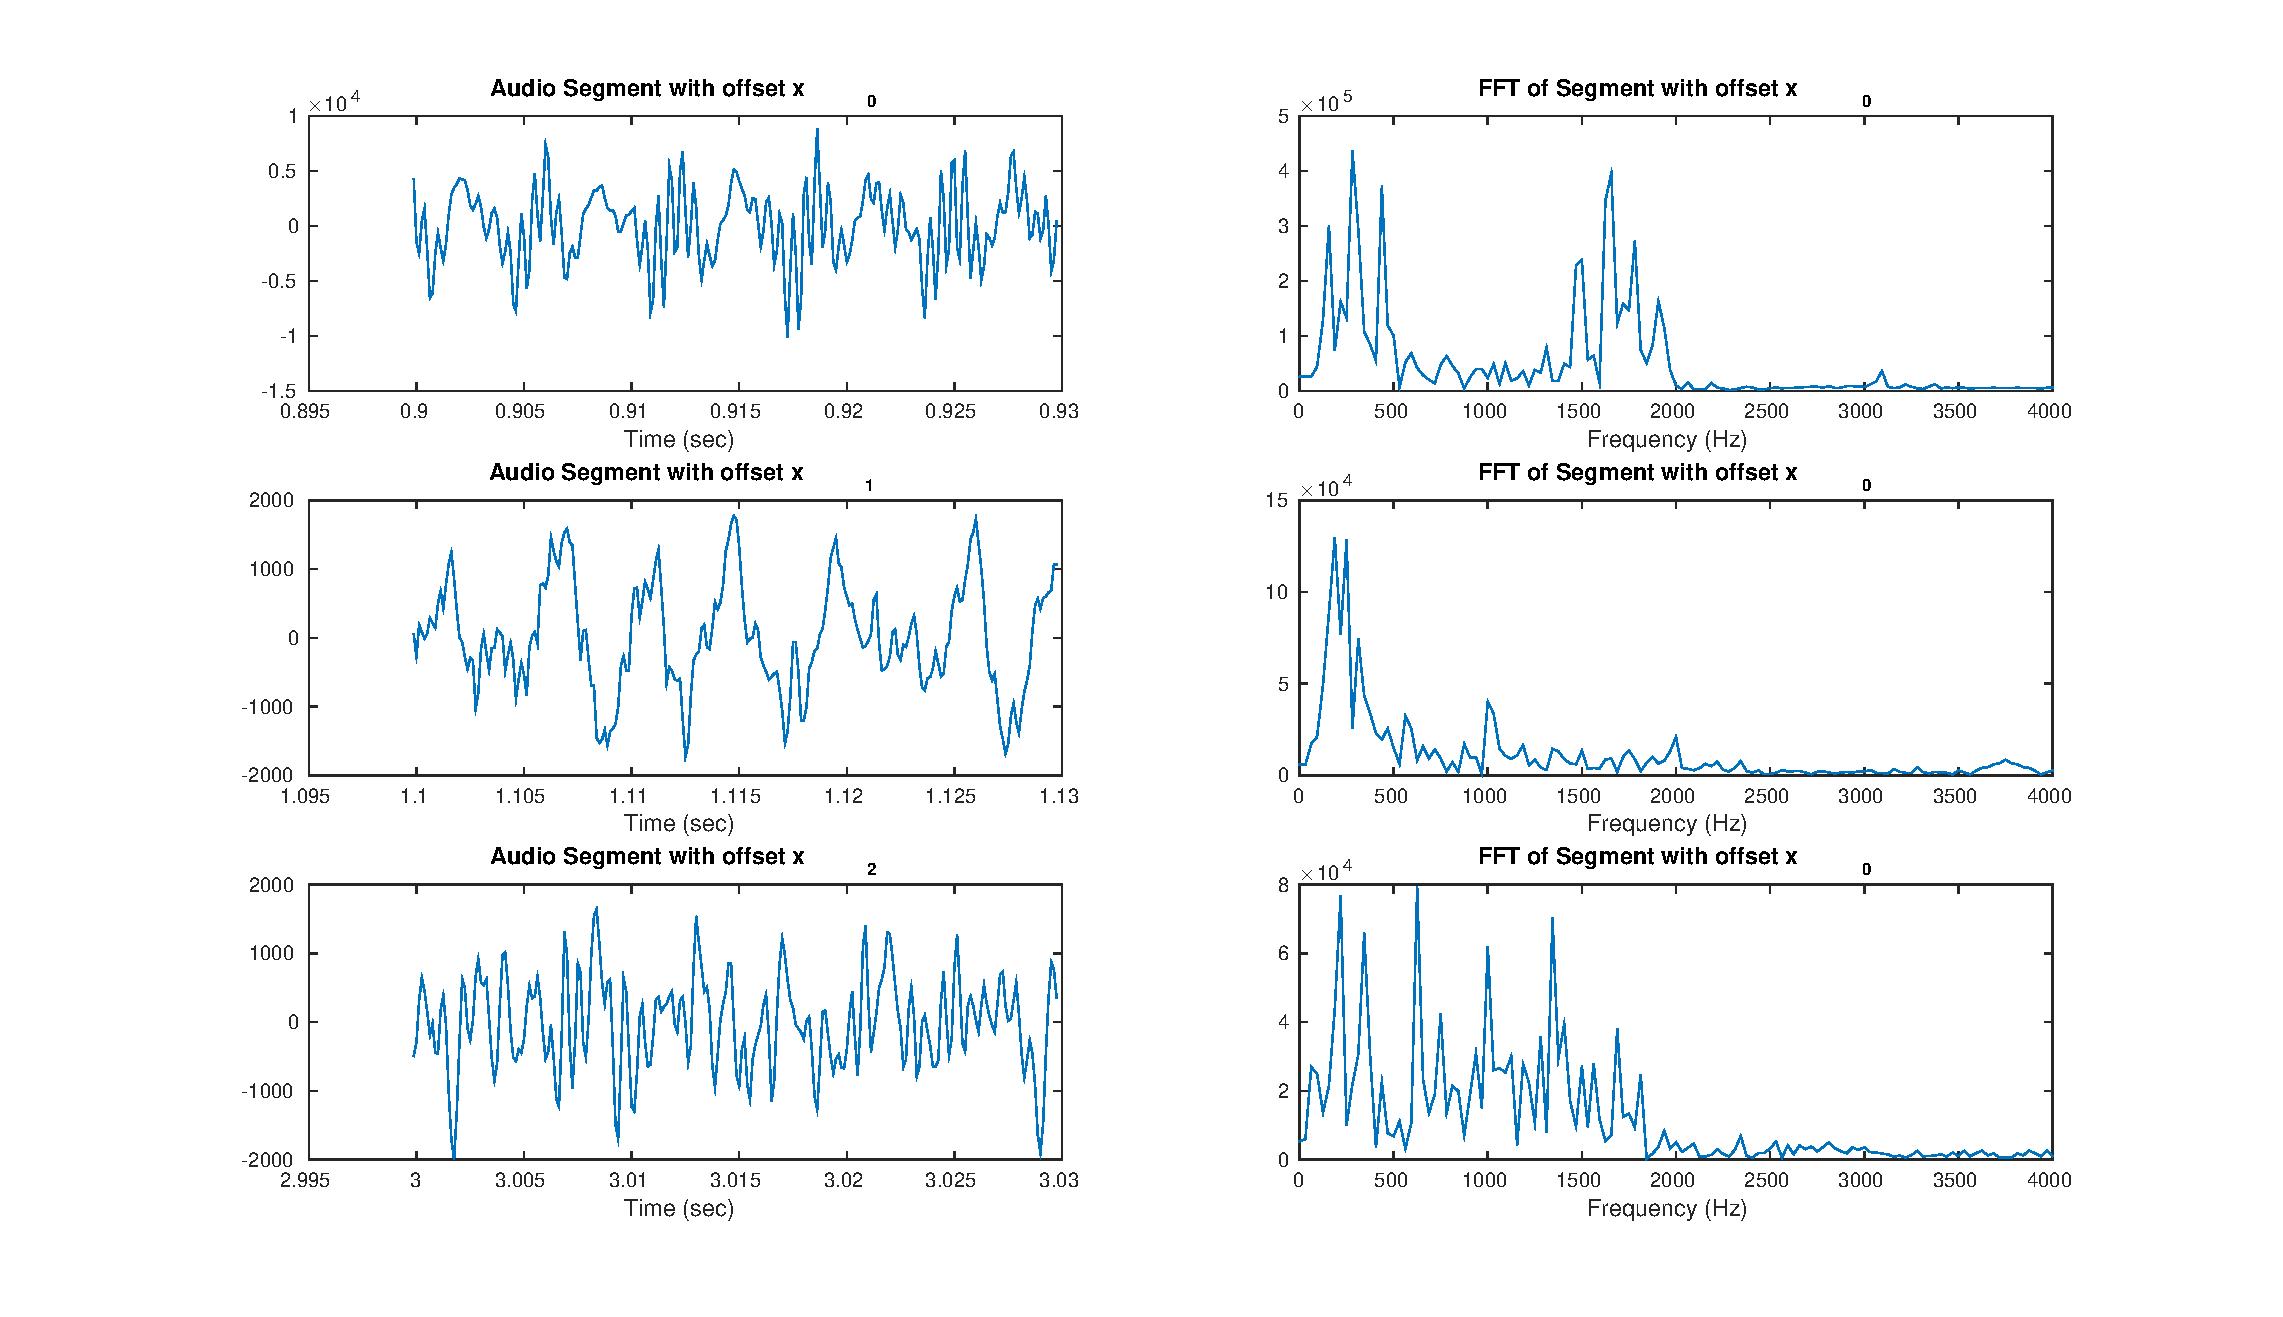
\includegraphics[width=\linewidth]{plot_5.eps}
	\caption{}
	\label{fig: transform} 
\end{figure}

\section{MATLAB Code} 
%Show and briefly explain your MATLAB code.
\lstinputlisting[frame=single, caption='MATLAB solution for CA: 05.']{../MATLAB/ca_05.m}

\section{Conclusions} 
%Summarize what you found.
Correlation and covariance are interesting metrics which are utilized to track how effectively two random variables are linearly related. With some ingenuity, the second task illustrates how the covariance between each element of a vector can be calculated and from that properties of the signal could be possibly extrapolated such as the amount of noise. Despite this tiny revelation, it presents more questions than answers. Why is the first and second offset different? Why is the first offset oscillating?  How exactly does the covariance matrix calculation work? 

\end{document}